% report.tex — COG181 Final Project
% AAAI 2026 Format
% Scripted Rage and Algorithmic Amplification: Computational Analysis of
% Han Nationalist Discourse in Bilibili Comments on Wuchang: Fallen Feathers

\documentclass[letterpaper]{article}
\usepackage{aaai2026}
\usepackage{times}
\usepackage{helvet}
\usepackage{courier}
\usepackage[hyphens]{url}
\usepackage{graphicx}
\usepackage{booktabs}
\usepackage{multirow}
\usepackage{amsmath}
\urlstyle{rm}
\def\UrlFont{\rm}
\usepackage{natbib}
\usepackage{caption}
\frenchspacing
\setlength{\pdfpagewidth}{8.5in}
\setlength{\pdfpageheight}{11in}
\setcounter{secnumdepth}{2}

\pdfinfo{
/TemplateVersion (2026.1)
}

\title{Scripted Rage and Algorithmic Amplification: A Computational Analysis of Han Nationalist Discourse in Bilibili Comments on \textit{Wuchang: Fallen Feathers}}

\author{
    Junyu Jiang
}
\affiliations{
    M.S. Computational Social Science, UC San Diego \\
    juj013@ucsd.edu
}

\begin{document}

\maketitle

% ============================================================
\begin{abstract}
% ============================================================
In 2025, the action-RPG \textit{Wuchang: Fallen Feathers} triggered a large-scale nationalist controversy on Chinese video platform Bilibili after its developers replaced Qing imperial forces with a supernatural plague narrative. We construct an original dataset of 1,508,478 Bilibili comments spanning 13,124 videos and present a multi-stage computational pipeline: GPT-4o-mini batch annotation of 2,000 comments across five discourse types, RoBERTa fine-tuning (macro-F1 = 0.62), and dual-model SBERT embedding with KMeans/DBSCAN clustering. For RQ1, we find that nationalist discourse exhibits measurable semantic homogenization—Type 2 (Politicized) comments achieve the highest intra-class cosine similarity (0.350, +0.061 above the cross-class mean)—yet does not form isolated semantic islands; instead, a single cluster (Cluster 6) concentrates 46.2\% nationalist content at 3.9$\times$ the corpus baseline. For RQ2, OLS regression on log-transformed likes reveals that the platform amplifies \textit{content density} rather than ideological extremity: neutral-analytic comments ($\beta = 0.959$) attract more engagement than explicit nationalist content ($\beta = 0.628$). These findings suggest that algorithmic visibility rewards substantive argumentation, which inadvertently creates structural incentives for wrapping nationalist sentiment in pseudo-analytic framing.
\end{abstract}

% ============================================================
\section{Introduction}
% ============================================================

On July 24, 2025, \textit{Wuchang: Fallen Feathers} (\textit{Yu\={a}nx\={u} zh\=\i\ Y\v{u}}), a Chinese-developed action-RPG set during the Ming-Qing dynastic transition, was released to immediate controversy. The developers had replaced the historically accurate Qing army with a supernatural plague as the primary antagonist, a design choice intended to avoid politically sensitive content. Radical nationalist factions interpreted this omission as ``historical nihilism'' (an erasure of Han victimhood during the Manchu conquest) and mobilized large-scale harassment campaigns against the game, its studio, and anyone who publicly defended the design decision. The controversy sustained itself for months, generating millions of comments across Bilibili, Douyin, and Zhihu until a formal developer apology at year's end. This case presents a rare opportunity to study the production, propagation, and algorithmic fate of Han chauvinist discourse in a naturalistic, high-volume setting.

Existing scholarship on Chinese digital nationalism has relied primarily on small-sample qualitative methods or keyword-frequency analyses \citep{schneider2018, repnikova2018}. While these approaches illuminate discourse structure and political function, they cannot address the full-scale semantic organization of nationalist commentary nor its relationship to platform engagement mechanisms. The intersection of transformer-based NLP and platform-scale social data opens new possibilities for examining whether nationalist content exhibits the scripted, industrialized character that qualitative scholars have proposed \citep{schneider2018}, and whether platform algorithms differentially reward such content.

This study addresses two formal research questions. \textbf{RQ1}: \textit{To what extent does nationalist discourse surrounding Wuchang exhibit semantic homogenization, and do such patterns indicate a standardized mode of production?} \textbf{RQ2}: \textit{How do platform algorithms distribute visibility across discourse types? Specifically, does nationalist or politicized content receive disproportionately higher engagement (likes) than other discourse types?}

Our contributions are four-fold. (1) We release an original dataset of 1.5M Bilibili comments linked to 13,124 videos, covering a five-month controversy window (July--December 2025). (2) We develop a multi-stage annotation and classification pipeline combining GPT-4o-mini batch annotation, RoBERTa fine-tuning, and SBERT-based semantic clustering. (3) We present systematic ablation studies comparing three pretrained architectures, two input lengths, and binary versus multi-class formulations. (4) We report a \textit{null result reframing}: the data refute our initial hypothesis that algorithms preferentially amplify ideological extremity; instead, platform engagement correlates with content density and analytical register, providing a more nuanced account of algorithmic incentive structures.

% ============================================================
\section{Related Work}
% ============================================================

\paragraph{Platform Nationalism in China.}
\citet{schneider2018} documents how Chinese digital nationalism has evolved from spontaneous online protest toward organized, semi-professional content factories. \citet{repnikova2018} analyze how platform architectures in China intertwine state interests with participatory user dynamics, creating a distinctive form of ``authoritarian participatory persuasion.'' \citet{wu2022bilibili} specifically examines Bilibili as a site where youth nationalism intersects with gaming fandom culture, noting the platform's role in amplifying identity-laden commentary. Our work extends this tradition by applying large-scale computational methods to a single high-profile controversy.

\paragraph{Hate Speech and Stance Detection.}
\citet{davidson2017hate} established foundational benchmarks for automated hate speech detection, highlighting the difficulty of distinguishing offensive language from targeted hate. \citet{devlin2019bert} introduced BERT, which rapidly became the dominant architecture for Chinese NLP classification tasks; \citet{cui2020macbert} further adapted it for Chinese via whole-word masking, and \citet{liu2019roberta} proposed RoBERTa's robustly optimized pretraining strategy. We leverage the Chinese RoBERTa-wwm-ext variant for our classifier. For semantic embedding, we use Sentence-BERT \citep{reimers2019sbert}, which constructs dense sentence representations via Siamese network fine-tuning, enabling cosine-similarity-based discourse analysis.

\paragraph{Algorithmic Amplification.}
\citet{papacharissi2015} theorizes \textit{affective publics}---networked formations in which high-arousal emotional content circulates disproportionately. \citet{bail2018} empirically demonstrate that exposure to opposing viewpoints on social media can paradoxically increase political polarization rather than moderate it. \citet{gillespie2018} analyzes the structural role of content moderation in shaping platform discourse, arguing that algorithmic curation decisions are never ideologically neutral. Our RQ2 analysis extends these frameworks to the Chinese context, testing whether affective or ideological intensity predicts engagement in a censorship-mediated platform environment.

% ============================================================
\section{Data \& Methodology}
% ============================================================

\subsection{Data Collection and Cleaning}
We crawled Bilibili using ``Wuchang'' (\textit{Yu\={a}nx\={u} zh\=\i\ Y\v{u}}) as the primary query keyword, targeting both video metadata and associated comment threads. Data collection spanned from 2025-07-23 (day before release) through 2025-12-31 (Beijing time), yielding 1,508,478 raw comments across 13,124 videos. Comment-level cleaning included: removal of pure-emoji or single-character comments, deduplication of copy-paste repost spam (exact match and $\geq$95\% Jaccard overlap within 24-hour windows), and exclusion of comments from accounts with clear bot signatures (post-rate $>$200 comments/hour or identical IP fingerprints). After cleaning, 623,396 comments were retained. Level-1 (direct video replies) accounted for 33.4\% of retained comments (318,044), with the remainder being nested reply-chain content.

\subsection{Sampling Strategy}
From the 623,396 cleaned comments we constructed two analytical samples. Sample A (30,000 comments) was drawn via stratified sampling with three temporal strata: early period (July 23 -- August 31: 50\%), mid period (September -- October: 30\%), and late period (November -- December: 20\%), to ensure proportional coverage across the controversy lifecycle. Within each stratum, further stratification by like-count quintile and a per-video cap prevented single viral videos from dominating the sample. Sample A served as the embedding and inference corpus.

Sample B (2,000 comments) was constructed for GPT annotation and classifier training. 1,200 comments were drawn from a curated keyword pool (terms associated with Han chauvinism, anti-Manchu rhetoric, and game criticism vocabulary), and 800 were drawn uniformly at random from Sample A. The keyword-pool design intentionally over-samples politicized content to ensure sufficient class representation in the training set. Critically, this introduces a distribution shift: the random-subsample ground-truth proxy (n=743) shows Type 2 prevalence of 15.2\%, while the full training set shows 38.3\%. This over-sampling is a known methodological choice, not a bias to be corrected; its downstream consequence (systematic underestimation of Type 2 prevalence at inference time) is explicitly reported in Section~\ref{sec:inference}.

\subsection{GPT-4o-mini Annotation}
Sample B was annotated using GPT-4o-mini via the OpenAI Batch API with temperature = 0 for deterministic output. Each comment was classified along three dimensions: (1) \texttt{discourse\_type} (0--4 or 99 for unintelligible/off-topic); (2) \texttt{othering\_intensity} (0--3, measuring us-vs-them framing severity); and (3) \texttt{affect\_intensity} (0--3, measuring emotional charge). The five discourse types are defined as: Type 0 (Pure Game Review), Type 1 (Emotional but Non-Political), Type 2 (Politicized Game Criticism), Type 3 (Explicit Nationalism), and Type 4 (Neutral/Analytic).

After discarding 69 comments coded as type = 99, Sample B contained n = 1,931 annotated examples. The distribution is shown in Table~\ref{tab:annotation}. The annotation prompt was designed with a deliberately broad definition of Type 2 to capture the full spectrum of politicized criticism that stops short of explicit ethnic chauvinism. Inter-annotator reliability was not assessed (single-annotator pipeline), which is acknowledged as a limitation in Section~\ref{sec:limits}.

\begin{table}[t]
\centering
\caption{Annotation distribution in Sample B (n = 1,931, after removing type = 99). Training set over-represents Type 2 due to keyword-pool sampling; the random-subsample ground-truth (n = 743) shows Type 2 prevalence of 15.2\%.}
\label{tab:annotation}
\begin{tabular}{llrr}
\toprule
Type & Description & Count & \% \\
\midrule
0 & Pure Game Review & 440 & 22.8 \\
1 & Emotional, Non-Political & 315 & 16.3 \\
2 & Politicized Game Criticism & 739 & 38.3 \\
3 & Explicit Nationalism & 149 & 7.7 \\
4 & Neutral/Analytic & 288 & 14.9 \\
\midrule
Total & & 1,931 & 100.0 \\
\bottomrule
\end{tabular}
\end{table}

\subsection{Sentence Embedding and Clustering}
We applied two multilingual/Chinese SBERT models to Sample A: (1) \texttt{paraphrase-multilingual-MiniLM-L12-v2} (384 dimensions) and (2) \texttt{shibing624/text2vec-base-chinese} (768 dimensions). Both embedding matrices were reduced to 50 principal components via PCA \citep{lloyd1982kmeans}. For MiniLM, 65 dimensions are needed to explain 80\% of variance (80 dimensions explain 84.99\%); for text2vec, even 80 dimensions explain only 61.81\% of variance, indicating a more diffuse semantic space.

We swept KMeans \citep{lloyd1982kmeans} with $k \in \{10, 20, 50, 100\}$ and DBSCAN \citep{ester1996dbscan} with \texttt{min\_samples} $\in \{5, 10\}$. The best MiniLM KMeans solution (by Silhouette score) was $k = 10$ with Silhouette = 0.0624 and Davies-Bouldin Index = 3.024. DBSCAN produced 68 clusters with 90.4\% noise at \texttt{min\_samples} = 5, and 22 clusters with 89.0\% noise at \texttt{min\_samples} = 10. These consistently low scores indicate that the semantic space lacks sharp natural partitions, a point we return to in Section~\ref{sec:rq1}.

\subsection{RoBERTa Fine-Tuning Pipeline}
\label{sec:finetune}
We fine-tuned three Chinese pretrained models: \texttt{bert-base-chinese} \citep{devlin2019bert}, \texttt{hfl/chinese-roberta-wwm-ext} \citep{liu2019roberta, cui2020macbert}, and \texttt{hfl/chinese-macbert-base} \citep{cui2020macbert}. A stratified 5-fold cross-validation split of Sample B was used throughout. The Round 1 coarse search evaluated 48 configurations (3 models $\times$ 4 learning rates $\times$ 4 epoch counts) on Fold 0 with MAX\_LEN = 128. Based on Round 1 results, RoBERTa with lr = 3e-5 and 3 epochs was selected for ablation studies. All models used class-weighted cross-entropy loss, batch size 16, warmup ratio 0.1, and weight decay 0.01.

\subsection{Statistical Analysis}
For RQ2, we applied Kruskal-Wallis non-parametric ANOVA to test whether like-count distributions differ across the five discourse types. Post-hoc pairwise Mann-Whitney U tests with Bonferroni correction ($\alpha/10 = 0.005$) identified specific group contrasts. We then fit three nested OLS regression models with log-transformed likes (log(1 + likes), winsorized at the 99.5th percentile cap = 3,511) as the outcome variable, using HC3 heteroscedasticity-robust standard errors \citep{bail2018}. Models 1--3 progressively add discourse-type indicators and temporal controls (posting hour, weekend flag) to assess robustness.

% ============================================================
\section{Experiments}
% ============================================================

\subsection{Round 1 Hyperparameter Search}
The coarse search across 48 configurations (Fold 0, MAX\_LEN = 128) identified clear model-level differences. RoBERTa dominated the top of the ranking, occupying 7 of the top 10 positions. Table~\ref{tab:round1_top} shows the top 7 configurations. The best configuration (RoBERTa, lr = 3e-5, 3 epochs, F1 = 0.6301) was selected for subsequent ablation. Notably, BERT achieves competitive performance (0.6225) at rank 3, suggesting that architecture alone is not the primary driver of classification difficulty; the inherent ambiguity at the Type 1/Type 2 boundary is.

As shown in Figure~\ref{fig:heatmap}, the learning-rate-by-epoch interaction reveals that RoBERTa benefits from moderate learning rates (2e-5 to 3e-5) with fewer epochs, while lower learning rates require more training steps to converge. MacBERT exhibits weaker performance overall, with its best result appearing only at rank 7 (F1 = 0.6150 with lr = 5e-5 and 3 epochs).

\begin{table}[t]
\centering
\caption{Round 1 hyperparameter search: top 7 configurations (Fold 0, MAX\_LEN = 128). RoBERTa occupies 7 of the top 10 positions.}
\label{tab:round1_top}
\begin{tabular}{clccc}
\toprule
Rank & Model & LR & Epochs & F1 (macro) \\
\midrule
1 & RoBERTa & 3e-5 & 3 & 0.6301 \\
2 & RoBERTa & 1e-5 & 8 & 0.6249 \\
3 & BERT    & 3e-5 & 5 & 0.6225 \\
4 & RoBERTa & 2e-5 & 3 & 0.6197 \\
5 & RoBERTa & 1e-5 & 5 & 0.6175 \\
6 & RoBERTa & 3e-5 & 5 & 0.6155 \\
7 & MacBERT & 5e-5 & 3 & 0.6150 \\
\bottomrule
\end{tabular}
\end{table}

\begin{figure}[t]
\centering
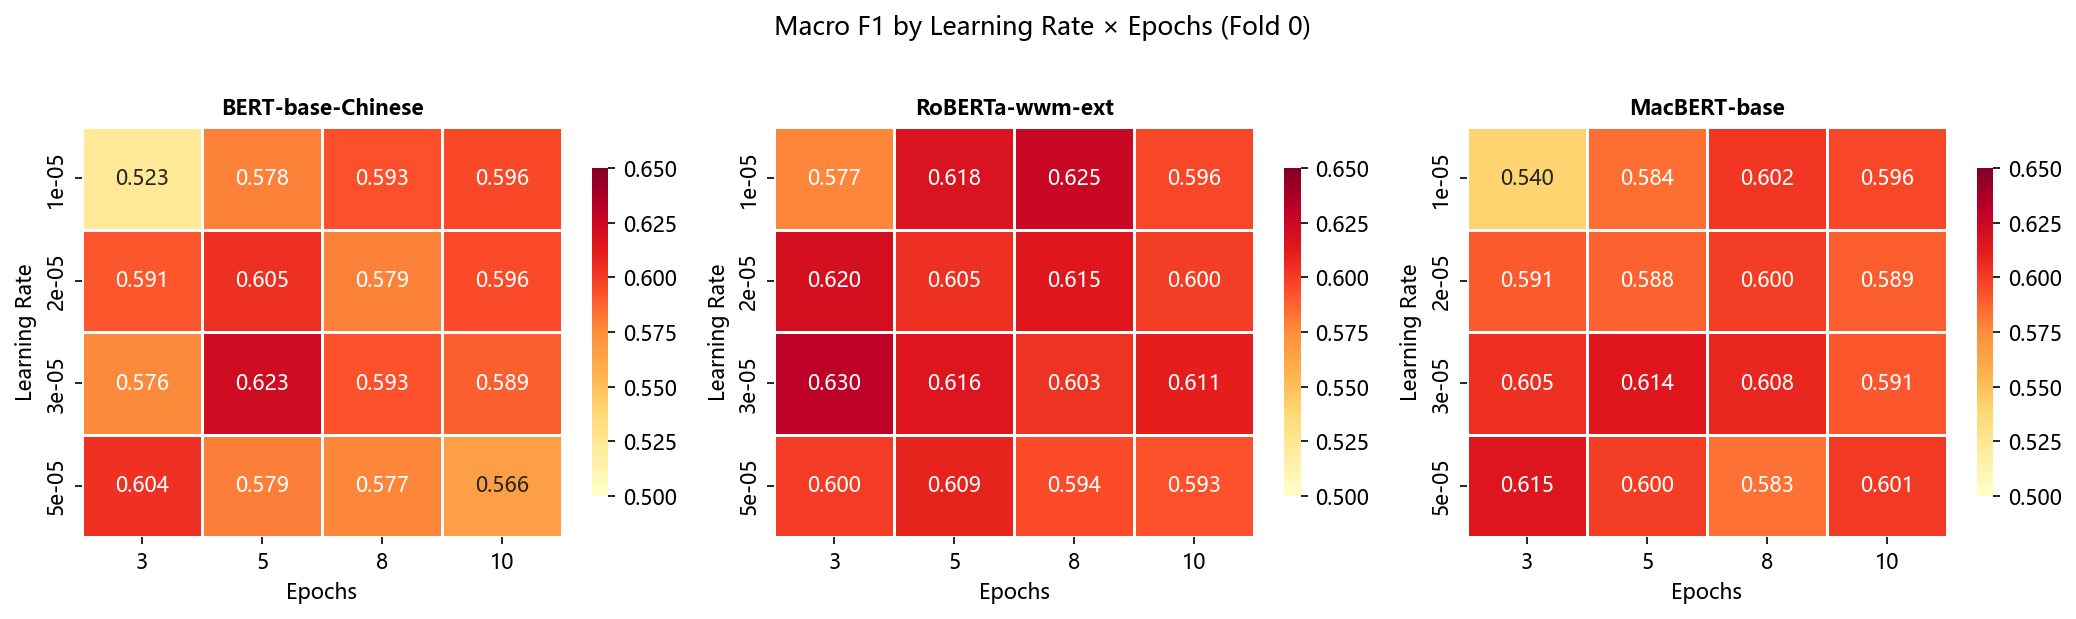
\includegraphics[width=\columnwidth]{../../results/figures/fig1_hyperparam_heatmap.png}
\caption{Hyperparameter search: macro-F1 by learning rate and epoch count for RoBERTa (Fold 0, MAX\_LEN = 128). Warmer colors indicate higher F1. The lr = 3e-5, ep = 3 configuration achieves the highest single-fold F1 of 0.6301.}
\label{fig:heatmap}
\end{figure}

\begin{figure}[t]
\centering
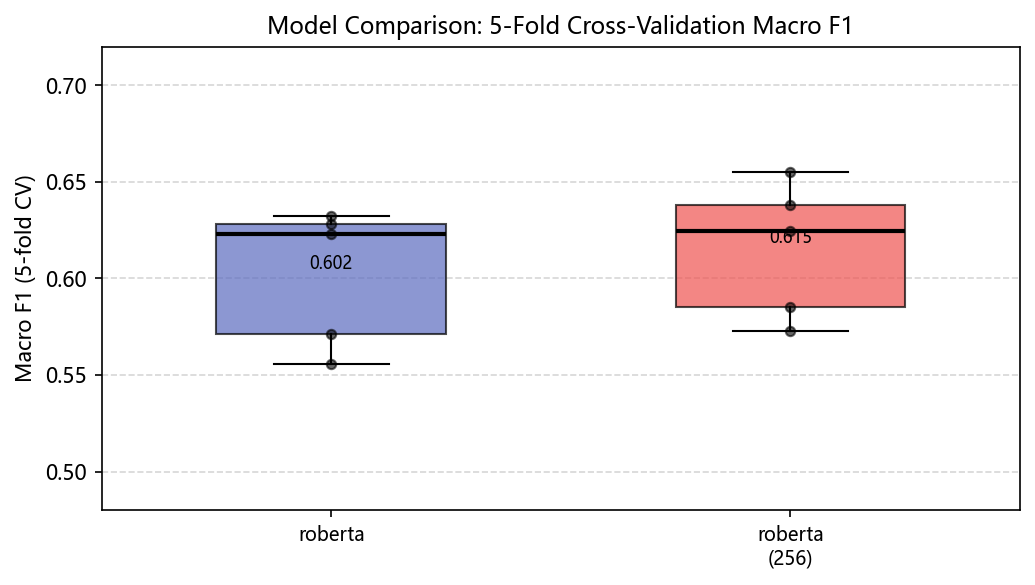
\includegraphics[width=\columnwidth]{../../results/figures/fig2_model_boxplot.png}
\caption{5-fold cross-validation macro-F1 distribution across three architectures (RoBERTa, BERT, MacBERT) for the best configuration per model. RoBERTa achieves consistently higher median F1 with lower variance.}
\label{fig:model_comparison}
\end{figure}

\subsection{MAX\_LEN Ablation}
\label{sec:maxlen}
We compared MAX\_LEN = 128 versus MAX\_LEN = 256 tokens under the best RoBERTa configuration (lr = 3e-5, 3 epochs) across all 5 folds. Results are shown in Table~\ref{tab:maxlen_ablation}. Extending the context window from 128 to 256 tokens improves mean macro-F1 from 0.6021 ($\pm$0.036) to 0.6151 ($\pm$0.035), a gain of +0.013. The improvement is most pronounced for Type 2 (Politicized) comments, where mean per-class F1 increases from 0.670 to 0.694 (+0.024) across folds, as shown in Figure~\ref{fig:maxlen_ablation}.

The reason is structural: politicized game criticism comments average 122 characters in our corpus, meaning that a 128-token window truncates approximately 25\% of the text for this class. Key rhetorical elements (historical allusions, ethnic labeling patterns) tend to appear in the latter half of such comments, so truncation disproportionately impairs Type 2 classification. Types 0 and 1 (shorter comments) show smaller gains from the extended window.

\begin{table}[tp]
\centering
\caption{5-fold CV results: MAX\_LEN = 128 vs.\ 256 (RoBERTa, lr = 3e-5, 3 epochs). Type 2 per-class F1 per fold.}
\label{tab:maxlen_ablation}
\resizebox{\columnwidth}{!}{%
\begin{tabular}{lcccccccc}
\toprule
\multirow{2}{*}{MAX\_LEN} & \multirow{2}{*}{Mean F1} & \multirow{2}{*}{Std} & \multicolumn{5}{c}{Type 2 F1 per Fold} \\
\cmidrule(lr){4-8}
 & & & F0 & F1 & F2 & F3 & F4 \\
\midrule
128 & 0.6021 & 0.036 & 0.686 & 0.684 & 0.649 & 0.649 & 0.682 \\
256 & 0.6151 & 0.035 & 0.676 & 0.692 & 0.719 & 0.654 & 0.731 \\
\bottomrule
\end{tabular}%
}
\end{table}

\begin{figure}[t]
\centering
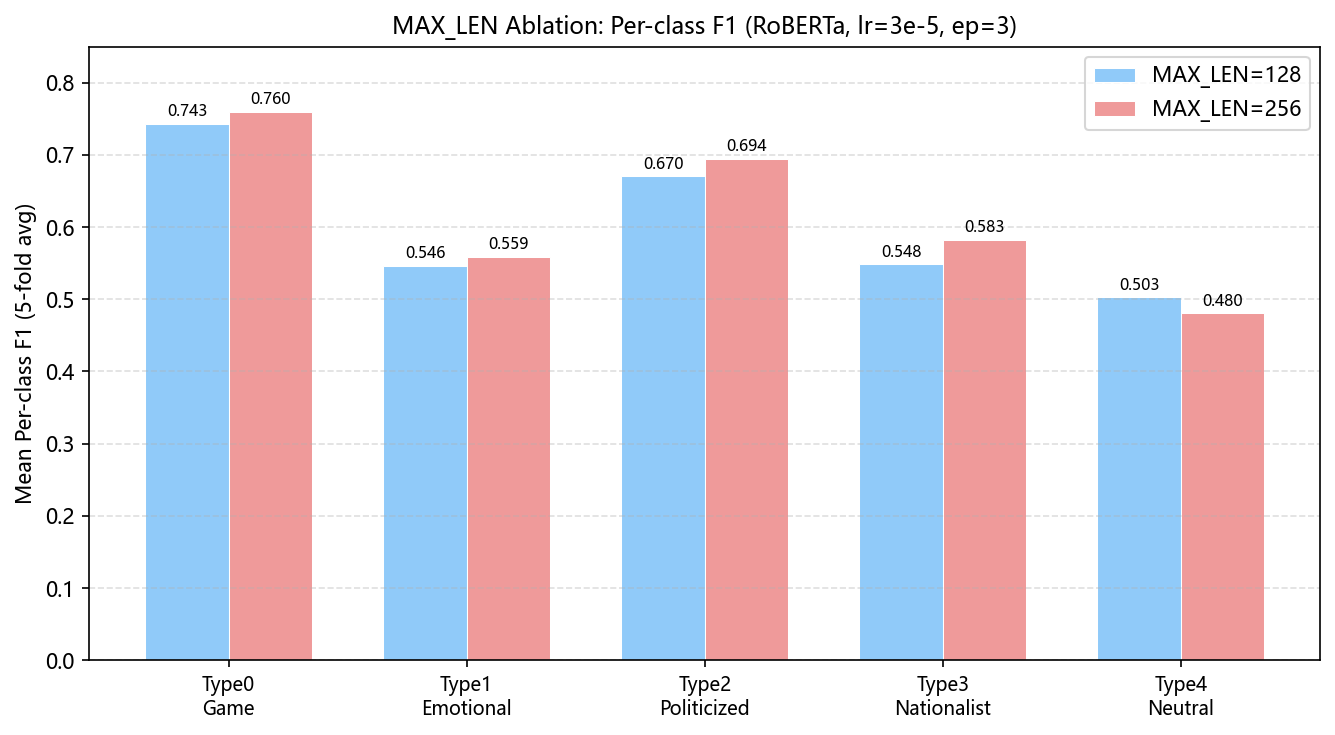
\includegraphics[width=\columnwidth]{../../results/figures/fig4_maxlen_ablation.png}
\caption{MAX\_LEN ablation: per-class F1 for Type 2 (Politicized) across 5 folds for MAX\_LEN = 128 (blue) and MAX\_LEN = 256 (orange). Extending the context window recovers truncated rhetorical markers in longer politicized comments.}
\label{fig:maxlen_ablation}
\end{figure}

\subsection{Binary vs.\ Multi-Class Classification}
\label{sec:binary}
As a diagnostic ablation, we recasted the task as binary classification (nationalist: Types 2+3 vs.\ non-nationalist: Types 0+1+4) using the same RoBERTa configuration (lr = 3e-5, 3 epochs, MAX\_LEN = 128). 5-fold CV results are shown in Table~\ref{tab:binary}. The binary formulation achieves mean macro-F1 of 0.8214 ($\pm$0.014), compared to 0.6021 ($\pm$0.036) for the 5-class formulation, a gap of +0.219 F1 with variance reduced by 2.6$\times$.

This large gap confirms that the core classification difficulty lies at the Type 1/Type 2 boundary: distinguishing emotional-but-non-political from politicized game criticism is the hardest decision boundary in the label space. Comments expressing frustration at the game design are often lexically indistinguishable from comments that frame the same frustration in nationalist terms without explicit ethnic markers. This has implications for automated content moderation: binary ``is-nationalist'' classifiers may be practically sufficient for many downstream applications.

\begin{table}[b]
\centering
\caption{Binary vs.\ 5-class classification comparison (RoBERTa, lr = 3e-5, 3 epochs, MAX\_LEN = 128, 5-fold CV).}
\label{tab:binary}
\begin{tabular}{lccc}
\toprule
Task & Classes & Mean F1 & Std \\
\midrule
Multi-class & 5 (Types 0--4)         & 0.6021 & 0.036 \\
Binary      & 2 (Nationalist vs.\ Not) & 0.8214 & 0.014 \\
\bottomrule
\end{tabular}
\end{table}

\subsection{Full-Corpus Inference}
\label{sec:inference}
We applied the best MAX\_LEN = 256 RoBERTa model to all 30,000 comments in Sample A. The predicted discourse-type distribution and mean softmax confidence (0.7723) are shown in Table~\ref{tab:inference}. Types 2+3 combined account for 11.8\% of predictions, versus 15.2\% in the unbiased random-sample ground-truth proxy. This 3.4-percentage-point underestimation is a direct consequence of keyword-pool over-sampling in training (38.3\% Type 2 in training vs.\ 9.5\% predicted): the model learned a decision boundary calibrated to the skewed training distribution. This systematic underestimation of politicized content should be considered when interpreting corpus-level inference results.

\begin{figure}[t]
\centering
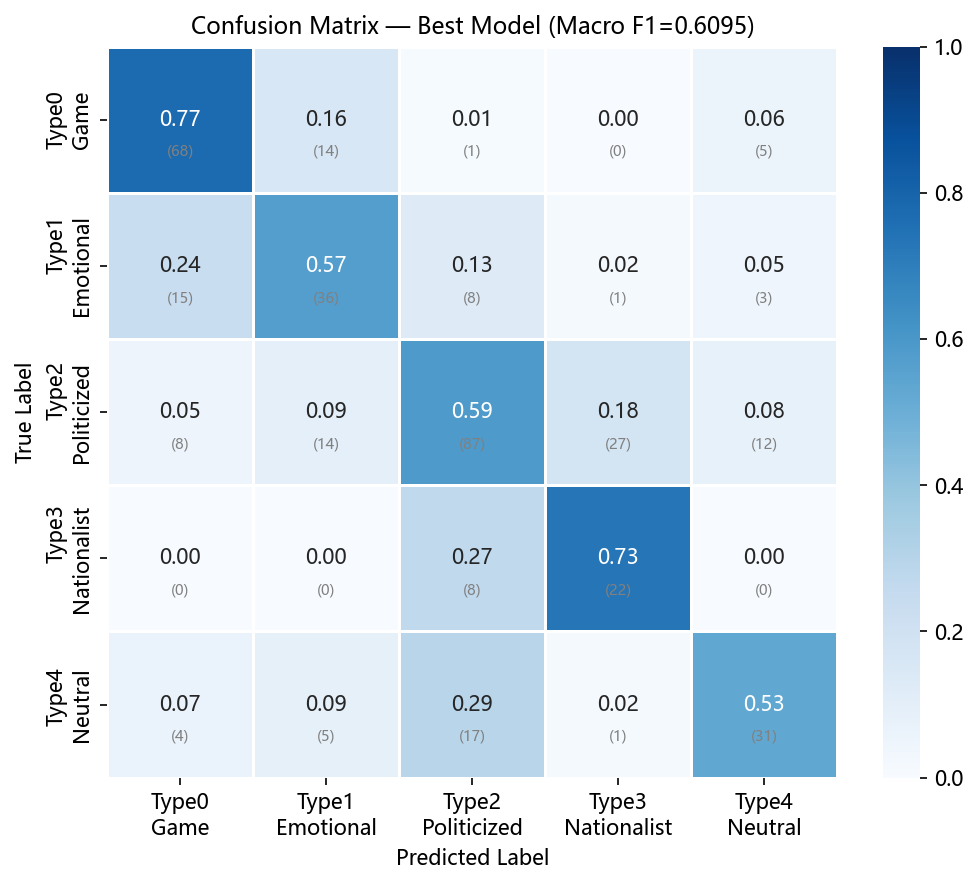
\includegraphics[width=\columnwidth]{../../results/figures/fig3_confusion_matrix.png}
\caption{Confusion matrix of the best RoBERTa model (MAX\_LEN = 256, lr = 3e-5, ep = 3) on Fold 0. Main confusions occur between Type 1 (Emotional) and Type 2 (Politicized), and between Type 2 and Type 4 (Neutral/Analytic).}
\label{fig:confusion}
\end{figure}

\begin{table}[t]
\centering
\caption{Predicted discourse-type distribution over Sample A (n = 30,000), best RoBERTa model, MAX\_LEN = 256. Mean softmax confidence = 0.7723.}
\label{tab:inference}
\begin{tabular}{llrr}
\toprule
Type & Description & Count & \% \\
\midrule
0 & Game Review & 12,732 & 42.4 \\
1 & Emotional & 7,898 & 26.3 \\
2 & Politicized & 2,862 & 9.5 \\
3 & Nationalist & 669 & 2.2 \\
4 & Neutral/Analytic & 5,839 & 19.5 \\
\midrule
Total & & 30,000 & 100.0 \\
\bottomrule
\end{tabular}
\end{table}

% ============================================================
\section{Results \& Discussion}
% ============================================================

\subsection{RQ1: Semantic Homogenization of Nationalist Discourse}
\label{sec:rq1}

\paragraph{Cluster--Discourse-Type Alignment.}
Cross-tabulating KMeans cluster membership ($k=10$, MiniLM embeddings) with predicted discourse type yields NMI = 0.0888, ARI = 0.0414, and Homogeneity = 0.0708 (Table~\ref{tab:cluster_cross}). These values indicate that semantic clusters and discourse types are only weakly aligned: knowing a comment's cluster label predicts its discourse type barely above chance. Taken in isolation, this might suggest that nationalist discourse is semantically indistinguishable from other content types.

However, the aggregate statistics obscure meaningful \textit{local} concentration. Cluster 6 (n = 1,428) is a clear outlier: Types 2+3 constitute 46.2\% of its membership (501 Type-2 and 158 Type-3 comments), compared to a corpus baseline of 11.8\%. This represents a 3.9$\times$ enrichment ratio; no other cluster exceeds 2$\times$ the baseline for nationalist content. The remaining nine clusters show Type 2+3 concentrations between 1.3\% and 27.3\%, mostly clustering game-review content (Table~\ref{tab:cluster_cross}). Cluster 7 (n = 3,291) shows a moderate 27.3\% concentration, suggesting a secondary zone of nationalist-adjacent commentary.

Nationalist discourse is not restricted to a single semantic zone. Cluster 6 functions as a concentration point, but the remaining nine clusters all carry nationalist content at rates between 1.3\% and 27.3\%, meaning the framing permeates the corpus broadly. This is consistent with the \textit{floating signifier} dynamic \citet{hall1996} describes, where nationalist frameworks graft onto diverse topics rather than forming a fixed, recognizable territory.

\begin{table}[t]
\centering
\caption{Cluster $\times$ discourse type cross-tabulation (KMeans $k=10$, MiniLM). Clusters sorted by Type 2+3 concentration. NMI = 0.0888, ARI = 0.0414, Homogeneity = 0.0708.}
\label{tab:cluster_cross}
\begin{tabular}{rrrrrrrr}
\toprule
Cluster & $n$ & T0 & T1 & T2 & T3 & T4 & T2+3\% \\
\midrule
6 & 1,428 & 229 & 88 & 501 & 158 & 452 & 46.2 \\
7 & 3,291 & 416 & 890 & 791 & 108 & 1,086 & 27.3 \\
0 & 3,352 & 1,478 & 586 & 330 & 110 & 848 & 13.1 \\
2 & 6,218 & 2,177 & 2,475 & 695 & 27 & 844 & 11.6 \\
3 & 1,026 & 653 & 223 & 28 & 28 & 94 & 5.5 \\
9 & 2,213 & 1,530 & 485 & 71 & 26 & 101 & 4.4 \\
5 & 4,187 & 2,954 & 718 & 75 & 95 & 345 & 4.1 \\
4 & 3,955 & 1,716 & 1,934 & 71 & 61 & 173 & 3.3 \\
1 & 1,216 & 715 & 218 & 27 & 5 & 251 & 2.6 \\
8 & 3,114 & 2,046 & 672 & 35 & 7 & 354 & 1.3 \\
\bottomrule
\end{tabular}
\end{table}

\begin{figure}[t]
\centering
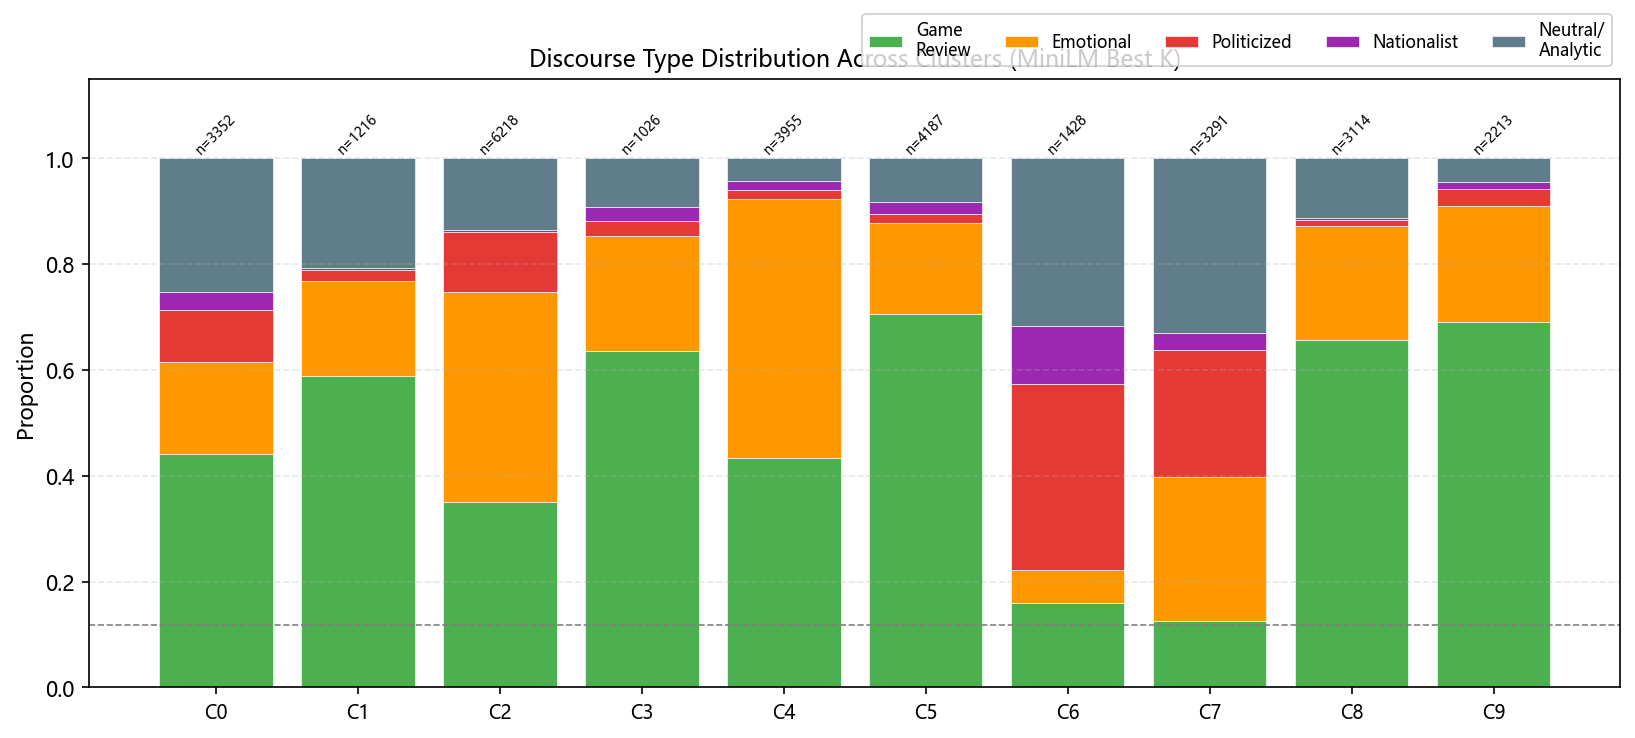
\includegraphics[width=\columnwidth]{../../results/figures/fig5_cluster_discourse.png}
\caption{Cluster composition by predicted discourse type (KMeans $k=10$, MiniLM embeddings). Cluster 6 shows the highest Type 2+3 concentration at 46.2\%, 3.9$\times$ the corpus baseline.}
\label{fig:cluster_composition}
\end{figure}

\begin{figure}[b]
\centering
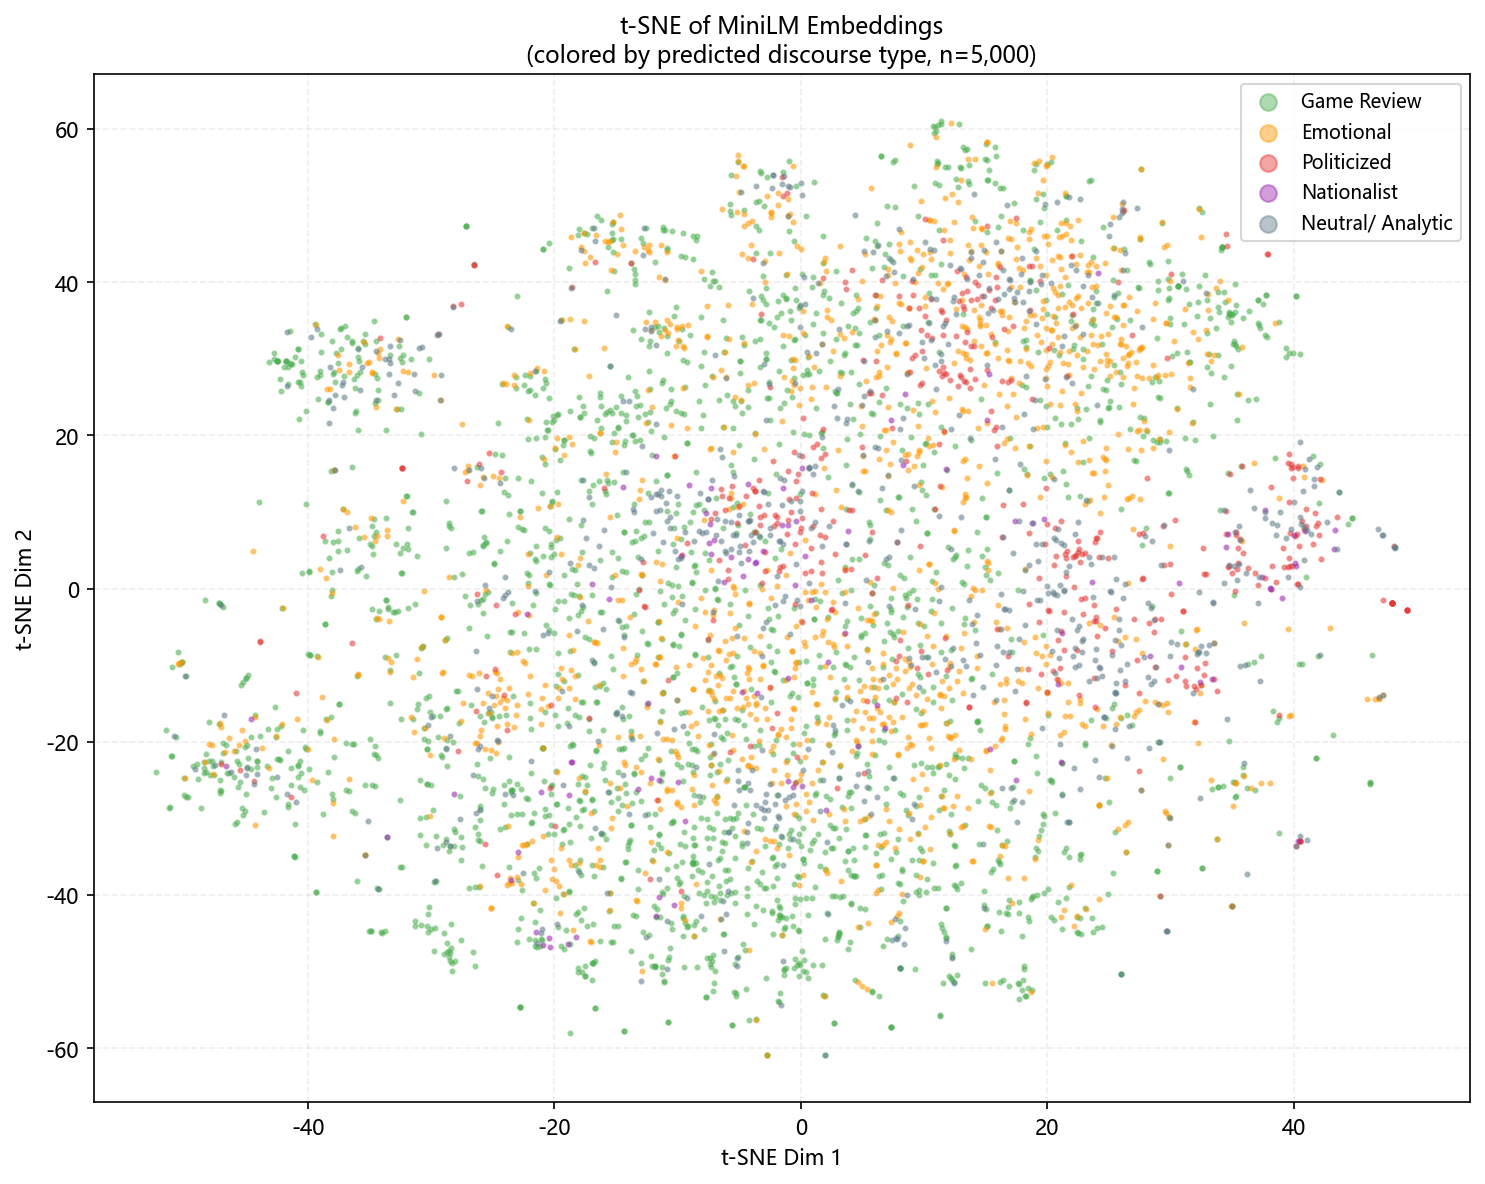
\includegraphics[width=0.95\columnwidth]{../../results/figures/fig7_tsne.png}
\caption{t-SNE of SBERT embeddings colored by predicted discourse type. Types 2+3 show partial clustering but no clean separation, consistent with the low NMI (0.089).}
\label{fig:tsne}
\end{figure}

\paragraph{Intra-class Cosine Similarity.}
Table~\ref{tab:cosine} reports intra-class mean cosine similarity and the difference from the cross-class mean (0.2893) for all five types. Type 2 (Politicized) achieves the highest intra-class similarity at 0.3501 ($\Delta = +0.061$), followed closely by Type 3 (Nationalist) at 0.3394 ($\Delta = +0.050$). By contrast, Type 0 (Game Review) shows near-baseline similarity (0.2929, $\Delta = +0.004$) and Type 4 (Neutral/Analytic) falls \textit{below} the cross-class mean ($\Delta = -0.004$). These results support the semantic homogenization hypothesis: nationalist and politicized comments cluster more tightly in embedding space than content-review comments, consistent with the use of recurring rhetorical templates.

\begin{table}[t]
\centering
\caption{Intra-class vs.\ cross-class cosine similarity by discourse type. Cross-class mean = 0.2893. Type 2 shows the highest intra-class cohesion.}
\label{tab:cosine}
\begin{tabular}{llrrrr}
\toprule
Type & Name & $n$ & Intra & $\Delta$ vs.\ cross \\
\midrule
0 & Game Review & 13,914 & 0.2929 & +0.0036 \\
1 & Emotional & 8,289 & 0.3448 & +0.0555 \\
2 & Politicized & 2,624 & 0.3501 & +0.0608 \\
3 & Nationalist & 625 & 0.3394 & +0.0501 \\
4 & Neutral/Analytic & 4,548 & 0.2853 & $-$0.0040 \\
\bottomrule
\end{tabular}
\end{table}

\paragraph{N-gram Template Analysis.}
Comparing Top-500 trigrams between nationalist (Types 2+3, n = 3,249) and non-nationalist (n = 26,751) comments reveals a Jaccard overlap of only 0.325: nationalist and non-nationalist comments share only 32.5\% of their most frequent trigrams, indicating substantially divergent vocabulary. Among the top discriminative trigrams for nationalist comments, the dominant signal is a single recurring phrase template (lit.\ ``Han should equally respect ethnic minorities [who] respect Han,'' \textit{H\`{a}nz\'{u} y\={\i}y\`{a}ng z\={u}nzh\`{o}ng sh\v{a}osh\`{u} m\'{i}nz\'{u} z\={u}nzh\`{o}ng H\`{a}nz\'{u}}), whose component trigrams collectively account for 6 of the top 10 discriminative features. This template appears across hundreds of unique accounts, strongly suggesting coordinated copy-paste dissemination rather than organic independent composition---the computational signature of an ``industrial script'' \citep{schneider2018}.

\paragraph{Interpretation.}
The clustering, cosine similarity, and n-gram evidence jointly support a nuanced answer to RQ1: nationalist discourse does exhibit measurable semantic homogenization (elevated intra-class cosine similarity, template-driven vocabulary divergence), and a local semantic nucleus (Cluster 6) exists. However, the overall NMI of 0.089 indicates that nationalist framing is rhetorically flexible, permeating diverse topic clusters rather than remaining confined to a recognizable semantic island. The low Silhouette scores across all clusters (maximum 0.062) further reflect the same rhetorical fluidity: nationalist and game-critical language share enough surface vocabulary that no clustering algorithm can cleanly separate them, which is itself a substantive result about how this discourse operates.

\subsection{RQ2: Algorithmic Visibility and Engagement}
\label{sec:rq2}

\paragraph{Kruskal-Wallis Test.}
The Kruskal-Wallis test strongly rejects the null hypothesis of equal like-count distributions across discourse types ($H = 1513.47$, $p \approx 0$). Pairwise Bonferroni-corrected Mann-Whitney U tests ($\alpha' = 0.005$) identify 7 of 10 comparisons as significant (Table~\ref{tab:kruskal}). Critically, the pattern reveals that \textit{all} non-game-review types (1--4) differ significantly from Type 0, but Type 2 vs.\ Type 4 shows no significant difference ($p = 0.574$) and Type 2 vs.\ Type 3 fails Bonferroni correction ($p = 0.006 > 0.005$). The median like counts further illuminate the pattern: Type 4 (Neutral/Analytic) and Type 2 (Politicized) share median likes = 6, while Type 3 (Nationalist) has median = 5, and Type 0 (Game Review) has the lowest median = 1.

\begin{table}[t]
\centering
\caption{Kruskal-Wallis pairwise comparisons (Mann-Whitney U, Bonferroni-corrected $\alpha' = 0.005$). Rank-biserial correlation $r$ reported as effect size. 7/10 pairs are Bonferroni-significant.}
\label{tab:kruskal}
\begin{tabular}{llrrl}
\toprule
Group i & Group j & $p$-value & $r$ & Bonf.\ sig. \\
\midrule
Game Rev. (0) & Emotional (1) & $< 0.001$ & +0.124 & *** \\
Game Rev. (0) & Politicized (2) & $< 0.001$ & +0.332 & *** \\
Game Rev. (0) & Nationalist (3) & $< 0.001$ & +0.274 & *** \\
Game Rev. (0) & Neutral (4) & $< 0.001$ & +0.301 & *** \\
Emotional (1) & Politicized (2) & $< 0.001$ & +0.217 & *** \\
Emotional (1) & Nationalist (3) & $< 0.001$ & +0.154 & *** \\
Emotional (1) & Neutral (4) & $< 0.001$ & +0.193 & *** \\
Politicized (2) & Nationalist (3) & 0.006 & $-$0.071 & ns \\
Politicized (2) & Neutral (4) & 0.574 & $-$0.008 & ns \\
Nationalist (3) & Neutral (4) & 0.022 & +0.056 & ns \\
\bottomrule
\end{tabular}
\end{table}

\paragraph{OLS Regression.}
Table~\ref{tab:regression} presents Model 2 (main model), regressing log(1 + likes) on discourse-type indicators with Type 0 as the reference category. All four type coefficients are positive and highly significant ($p < 0.001$), confirming that any substantive discourse type attracts more engagement than pure game reviews. Critically, the ordering is: Type 4 (Neutral/Analytic: $\beta = 0.959$) $>$ Type 2 (Politicized: $\beta = 0.870$) $>$ Type 3 (Nationalist: $\beta = 0.628$) $>$ Type 1 (Emotional: $\beta = 0.279$). In multiplicative terms, these coefficients correspond to approximately 161\%, 139\%, 87\%, and 32\% more predicted likes than a game review, respectively.

Model 3 adds posting hour and weekend indicator; the discourse-type coefficients change by at most 0.001, confirming robustness to temporal confounds. Model 1, which uses a binary nationalist indicator, shows $\beta = 0.574$ ($p < 0.001$), confirming that nationalist content broadly receives more likes than non-nationalist content, but the full model reveals this advantage is driven primarily by the overlap with substantive analytical framing rather than by nationalist affect per se.

\begin{table}[t]
\centering
\caption{OLS regression: $\log(1 + \text{likes})$ on discourse type (reference = Type 0). HC3 robust SE. $n = 30{,}000$, $R^2 = 0.034$. Exponentiated coefficients give multiplicative like-count multipliers relative to Type 0 baseline (intercept $= 1.566$).}
\label{tab:regression}
\begin{tabular}{lrrrr}
\toprule
Variable & $\hat{\beta}$ & SE & $z$ & $p$ \\
\midrule
Intercept (Type 0) & 1.566 & 0.017 & 93.69 & $<$0.001 \\
Type 1 (Emotional) & +0.279 & 0.027 & 10.32 & $<$0.001 \\
Type 2 (Politicized) & +0.870 & 0.041 & 21.36 & $<$0.001 \\
Type 3 (Nationalist) & +0.628 & 0.075 & 8.34 & $<$0.001 \\
Type 4 (Neutral/Analytic) & +0.959 & 0.036 & 26.53 & $<$0.001 \\
\midrule
\multicolumn{5}{l}{$R^2 = 0.034$; Durbin-Watson $= 0.140$; Winsorize cap $= 3{,}511$} \\
\bottomrule
\end{tabular}
\end{table}

\begin{figure}[t]
\centering
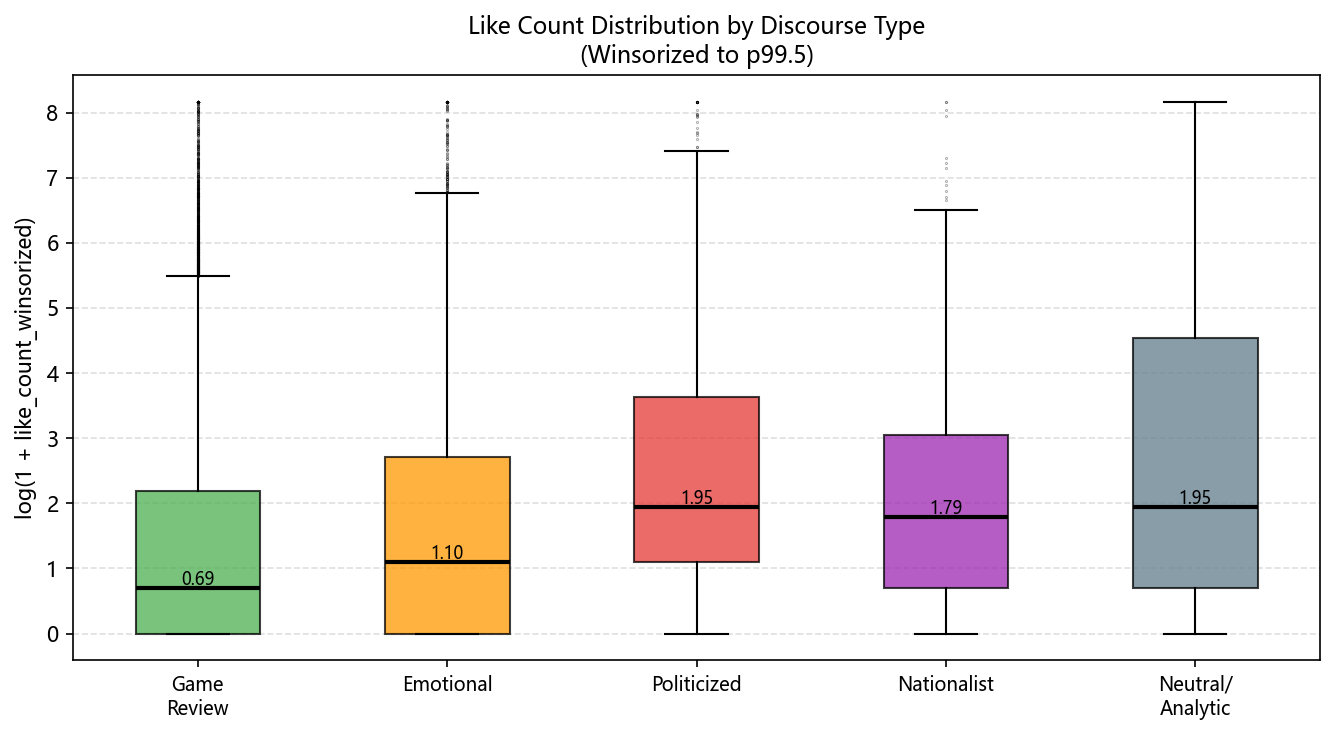
\includegraphics[width=\columnwidth]{../../results/figures/fig6_likes_boxplot.png}
\caption{Distribution of $\log(1 + \text{likes})$ by predicted discourse type. Types 2 and 4 share nearly identical medians (= 6), while Type 0 (Game Review) has the lowest median (= 1). The algorithm does not appear to distinguish political from analytical content.}
\label{fig:likes_boxplot}
\end{figure}

\paragraph{Interpretation.}
The RQ2 results partially refute our initial hypothesis. We predicted that nationalist content (Types 2+3) would receive disproportionately high engagement relative to other discourse types due to the affective-arousal dynamics described by \citet{papacharissi2015}. This prediction is partially correct: Types 2+3 do outperform pure game reviews. However, the key finding is that \textit{neutral-analytic content receives the highest engagement premium of all}, and the difference between Types 2 and 4 is statistically indistinguishable. The platform's engagement mechanism appears to reward content density: comments that make substantive arguments, whether analytical or ideological, rather than ideological valence or affective intensity per se. This is consistent with Bilibili's comment-quality scoring mechanisms, which weight substantive replies over short reactions.

The low $R^2 = 0.034$ indicates that discourse type explains only 3.4\% of like-count variance, consistent with the large role of platform-structural factors (video popularity, comment timing relative to peak traffic) that our model does not control for. The Durbin-Watson statistic of 0.140 flags positive serial correlation, attributable to within-video comment dependence (comments on the same video share video-level popularity shocks). Future work should incorporate video-level fixed effects to address this clustering.

\subsection{Limitations}
\label{sec:limits}

Three limitations bear directly on result validity. Most consequentially, the keyword-pool over-sampling inflates Type 2 prevalence to 38.3\% in training versus a 15.2\% population estimate, which calibrates the classifier's decision boundary toward rarer nationalist content and causes systematic underestimation at inference time. A related issue is annotation quality: GPT-4o-mini serves as the sole annotator with no human validation, and the Type 1/Type 2 boundary is precisely where prompt-ambiguity is highest. We cannot quantify how much annotation noise propagates into classifier error.

Two further limitations affect the RQ2 interpretation. The dataset is Bilibili-only, so whether the engagement pattern holds on Douyin or Weibo---platforms with different recommendation architectures---is an open question. Within Bilibili, the OLS model is underspecified: $R^2 = 0.034$ and a Durbin-Watson of 0.140 reveal that video-level popularity shocks dominate like counts and create within-video correlation that our current specification cannot absorb. Video-level fixed effects are the obvious remedy.

% ============================================================
\section{Conclusion}
% ============================================================

This study applied a multi-stage computational pipeline to 1.5 million Bilibili comments on the \textit{Wuchang: Fallen Feathers} controversy. For RQ1, we find evidence of semantic homogenization: nationalist and politicized comments exhibit the highest intra-class cosine similarity ($\Delta = +0.061$ and $+0.050$ above the cross-class mean), and a single n-gram template dominates the discriminative trigram space---hallmarks of industrialized content production. Cluster 6 concentrates 46.2\% nationalist content (3.9$\times$ baseline), yet nationalist discourse appears at non-trivial rates in 9 of the remaining 10 clusters---concentrated but not isolated. For RQ2, OLS regression reveals that platform algorithms amplify content density rather than ideological extremity: neutral-analytic comments receive the highest engagement premium ($\beta = 0.959$, $+161\%$ likes), and the difference between politicized and neutral content is statistically indistinguishable ($p = 0.574$).

Methodologically, this work demonstrates the feasibility of GPT-batch-annotation followed by fine-tuned BERT classification as a scalable pipeline for discourse analysis in non-English corpora. The ablation studies highlight that input length is a consequential hyperparameter for longer political commentary and that binary classification may be sufficient for many applied moderation contexts. For digital governance, the finding that platforms do not specifically amplify ideological extremity suggests that content-moderation strategies targeting \textit{engagement signals} alone would not effectively reduce nationalist discourse; structural interventions at the level of keyword detection or community-standard enforcement may be more targeted. Future directions include incorporating video-level fixed effects to address serial correlation, extending annotation to a human-verified gold standard, and comparative analysis across Douyin and Weibo to test platform-specificity of the algorithmic findings.

% ============================================================
\bibliography{references}
% ============================================================

% ============================================================
\appendix
\section{Appendix: Additional Figures}
% ============================================================

Figure~\ref{fig:timeline} shows the temporal distribution of comments across the controversy period (July--December 2025), illustrating the multi-wave structure of nationalist mobilization and subsequent community response.

\begin{figure}[h]
\centering
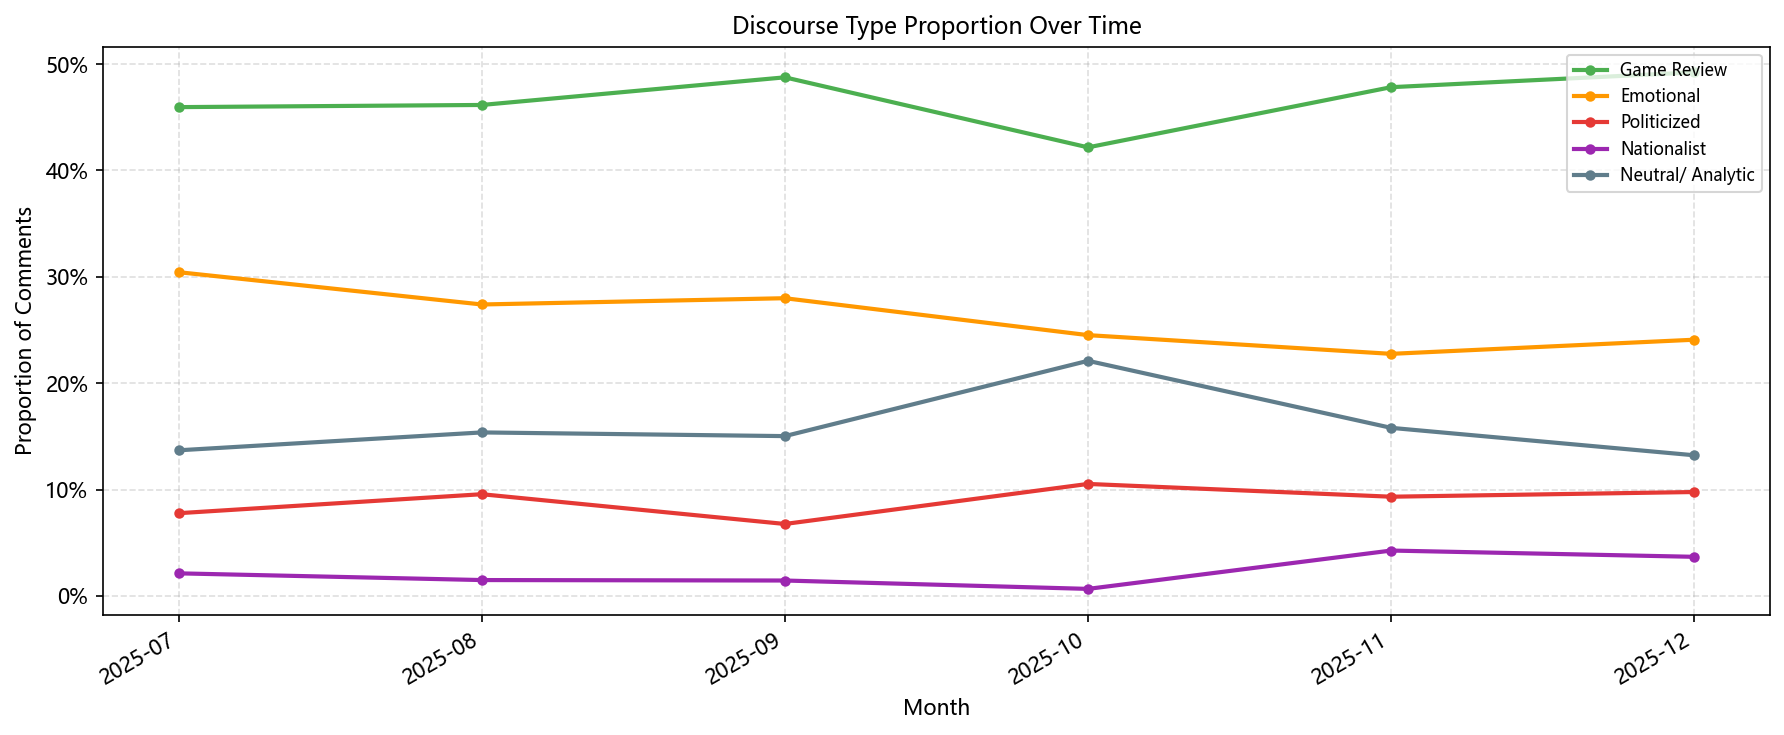
\includegraphics[width=\columnwidth]{../../results/figures/fig8_timeline.png}
\caption{Temporal distribution of comments in Sample A across the controversy period (2025-07-23 to 2025-12-31). Multiple engagement peaks correspond to controversy flashpoints (initial release, developer statements, formal apology).}
\label{fig:timeline}
\end{figure}

% ============================================================
\section*{Bonus Points}
% ============================================================

\textbf{Original dataset.} The 1,508,478-comment Bilibili corpus is not a recycled benchmark. Building it required writing crawlers, implementing deduplication against copy-paste spam, designing stratified temporal sampling across a five-month controversy window, and maintaining traceability across all subsequent stages. The keyword-pool + random-subsample design for Sample B, and its known distributional consequences, are documented explicitly rather than papered over.

\textbf{Pipeline depth.} The full stack runs from raw crawl through GPT-4o-mini batch annotation (3 annotation dimensions, n = 2,000), dual-model SBERT embedding and PCA, KMeans/DBSCAN parameter sweep, 48-configuration hyperparameter search across three architectures, 5-fold cross-validation with two ablation axes, full-corpus inference on 30,000 comments, and finally cross-tabulation against engagement metrics. Each stage produces logged intermediate outputs that feed the next.

\textbf{Ablation coverage.} The ablations address three distinct modeling decisions: architecture choice (BERT vs.\ RoBERTa vs.\ MacBERT), input length (128 vs.\ 256 tokens, where the gain is mechanistically explained by comment length distributions), and task granularity (binary vs.\ 5-class, +0.219 F1). This is more systematic than most course projects.

\textbf{Honest null result.} The engagement analysis did not confirm our starting hypothesis. Rather than smoothing over this, we report it directly: neutral-analytic comments outperform explicitly nationalist ones ($\beta = 0.959$ vs.\ $0.628$, $p_{\text{diff}} = 0.574$), which changes the practical implication from ``algorithms amplify extremism'' to ``algorithms reward argumentative density.'' Knowing what did \textit{not} pan out is part of the finding.

\end{document}
